\section{Matriser av godtycklig storlek (Avs 4.2)}
\paragraph{Definition} En \underline{$m\times n$-matris} är ett tvådimensionellt fält med reella tal som har $m$ rader och $n$ kolumner.
\begin{equation*}
    A=\begin{pmatrix}
        a_{1,1} & a_{1,2} & \ldots & a_{1,n}\\
        a_{2,1} & a_{2,2} & \ldots & a_{2,n}\\
        \vdots & \vdots & \ddots & \vdots\\
        a_{m,1} & a_{m,2} & \ldots & a_{m,n}
    \end{pmatrix} = \begin{pmatrix}
        \bm{a}_{1} & \bm{a}_{2} & \ldots & \bm{a}_{n}
    \end{pmatrix}
\end{equation*}

Addition av matriser går till som tidigare och det gör även multiplikation med ett tal.
Om $A$ är en matris med talet $a_{i,j}$ på plats $(i,j)$ då är $A^{t}$, transponatet av $A$, matrisen med tal $a_{j,i}$ på plats $(i,j)$.
\begin{equation*}
    A^{t}=\begin{pmatrix}
        a_{1,1} & a_{2,1} & \ldots & a_{m,1}\\
        a_{1,2} & a_{2,2} & \ldots & a_{m,2}\\
        \vdots & \vdots & \ddots & \vdots\\
        a_{1,n} & a_{2,n} & \ldots & a_{m,n}
    \end{pmatrix}
\end{equation*}
Om $A$ är $m\times n$-matris sår är $A^{t}$ $n\times m$-matris.

\paragraph{Definition} Om $A$ är en $m\times n$-matris och $\bm{v}$ är en $n$-vektor så låter vi 
\begin{equation*}
    A\bm{v}=\begin{pmatrix}
        \bm{a}_{1}&\bm{a}_{2}& \ldots &\bm{a}_{n}
    \end{pmatrix}\begin{pmatrix}
        v_{1}\\ v_{2}\\ \vdots \\ v_{n}
    \end{pmatrix}=v_{1}\bm{a}_{1}+v_{2}\bm{a}_{2}+\ldots+v_{n}\bm{a}_{n}
\end{equation*}
Observera att $A\bm{v}$ är en $m$-vektor!

\paragraph{Definition} Om $A$ är en $m\times n$-matris och $B$ är en $n\times p$-matris då låter vi 
\begin{equation*}
    AB-A\begin{pmatrix}
        \bm{b}_{1}& \bm{b}_{2} &\ldots&\bm{b}_{p}
    \end{pmatrix}=\begin{pmatrix}
        A\bm{b}_{1}& A\bm{b}_{2} & \ldots &A\bm{b}_{p}
    \end{pmatrix}
\end{equation*}
Observera att $AB$ är en $m\times p$-matris.

\paragraph{Proposition 4.21} Låt $A$ vara $m\times n$-matris och $B$ en $n\times p$-matris och låt $C=AB$.
Då ges $c_{i,j}$, elementet på plats $(i,j)$ för $C$, av 
\begin{equation*}
    c_{i,j}=\sum_{k=1}^{n}a_{i,k}b_{kj}
\end{equation*}

\paragraph{Proposition 4.23} Om $A=\begin{pmatrix}\bm{r}^{t}_{1}\\\bm{r}^{t}_{2}\\\vdots\\\bm{r}^{t}_{m}\end{pmatrix}$ och 
$B=\begin{pmatrix}\bm{b}_{1}&\bm{b}_{2}&\ldots&\bm{b}_{p}\end{pmatrix}$ då är 
\begin{equation*}
        AB=\begin{pmatrix}
        \bm{r}^{t}_{1}\bm{b}_{1} & \bm{r}^{t}_{1}\bm{b}_{2} & \ldots & \bm{r}^{t}_{1}\bm{b}_{p}\\
        \bm{r}^{t}_{2}\bm{b}_{1} & \bm{r}^{t}_{2}\bm{b}_{2} & \ldots & \bm{r}^{t}_{2}\bm{b}_{p}\\
        \vdots & & & \vdots\\
        \bm{r}^{t}_{m}\bm{b}_{1}
    \end{pmatrix}
\end{equation*}

~\\

Det finns flera naturliga räkneregler för addition och multiplikation av matriser men fortfarande är $AB\neq BA$ i allmänhet.

\paragraph{Proposition 4.25} Matrisen $I_{n}=\begin{pmatrix}\bm{e}_{1}&\bm{e}_{2}&\ldots&\bm{e}_{n}\end{pmatrix}$ är en identitetsmatris (för $n\times n$-matriser).
Dvs om $A$ är en $n\times n$ matris så är $AI_{n}=A=I_{n}A$.
En $n\times n$-matris $B$ är en invers till $n\times n$-matrisen $A$ om $AB=I_{n}=BA$.
Om det finns en invers så är den unik, så vi kan prata om inversen till A (om den finns).

\paragraph{Proposition 4.27} Om $A_{1}$, $A_{2}$, $\ldots $, $A_{m}$ är inverterbara då är $A_{1}\cdot A_{2}\cdot \ldots \cdot A_{m}$ inverterbar och 
$(A_{1}A_{2}\ldots A_{m})^{-1}=A_{m}^{-1}\ldots A_{2}^{-1}A_{1}^{-1}$

\section{Linjära avbildningar från $\mathbb{R}^{n}$ till $\mathbb{R}^{m}$ (Avs 4.2)}
En funktion $f:\mathbb{R}^{n}\rightarrow \mathbb{R}^{m}$ sägs vara linjär om 
\begin{enumerate}
    \item[] $f(\bm{u}+\bm{v})=f(\bm{u})+f(\bm{v})$ $\forall \bm{u},\bm{v}\in \mathbb{R}^{n}$
    \item[] $f(c\bm{v})=cf(\bm{v})$ $\forall c\in\mathbb{R},\bm{v}\in\mathbb{R}^{n}$
\end{enumerate}
Givet en $m\times n$-matris $A$ så får vi en linjär avbildning $f_{A}:\mathbb{R}^{m}\rightarrow \mathbb{R}^{n}$.
Genom $f_{A}(\bm{v})=A\bm{v}$.
Vi tänker ofta på matrisen som avbildningen och struntar då i notationen $f_{A}$.

\paragraph{Sats (Bassatsen)} Om $f:\mathbb{R}^{m}\rightarrow \mathbb{R}^{n}$ är en linjär avbildning då är $f$ en matrisavbildning med matrisen
\begin{equation*}
    A=\begin{pmatrix}
        f(\bm{e}_{1})&f(\bm{e}_{2})&\ldots&f(\bm{e}_{m})
    \end{pmatrix}
\end{equation*}

\begin{wrapfigure}{r}{0.35\textwidth}
    \centering
    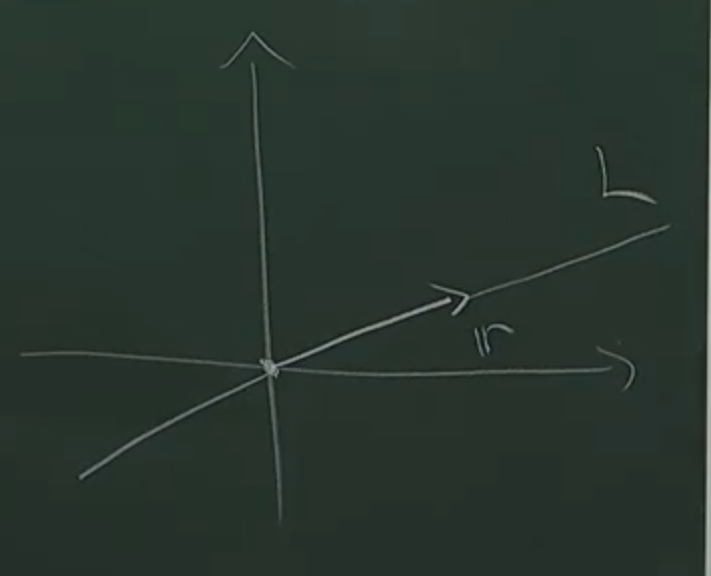
\includegraphics[scale=0.2]{imgs/img01.png}
\end{wrapfigure}
\paragraph{Ex} \underline{Ortogonal projektion på en linje}\\
I $\mathbb{R}^{n}$ ges en linje fortfarande av två punkter eller en punkt och en riktningsvektor $\bm{r}\neq \bm{0}$.
Om linjen går genom irgo $\bm{0}$ så kan vi välja punkten att vara origo och då behöver vi bara en riktningsvektor.
Den \underline{ortogonala projektionen av}
\underline{en vektor $\bm{v}\in \mathbb{R}^{n}$ på en linje $L$, riktningsvektor $\bm{r}$}\\
ges av $f_{L}(\bm{v})=\frac{\bm{v}\cdot \bm{r}}{\bm{r}\cdot \bm{r}}\bm{r}$.
Funktionen $F_{L}$ är linjär!
Matrisen till $f_{L}$ ges av: 
\begin{equation*}
    A=\begin{pmatrix}
        \frac{\bm{e}_{1}\cdot\bm{r}}{\bm{r}\cdot\bm{r}}\bm{r} & \frac{\bm{e}_{2}\cdot\bm{r}}{\bm{r}\cdot\bm{r}}\bm{r} & \ldots & \frac{\bm{e}_{n}\cdot\bm{r}}{\bm{r}\cdot\bm{r}}\bm{r}
    \end{pmatrix}
\end{equation*}
Avbildningen $A$ är alltså en avbildning från $\mathbb{R}^{n}$ till $\mathbb{R}^{n}$ men $A\bm{v}$ ligger på linjen $L$ för varje $\bm{v}\in\mathbb{R}^{n}$.

\chapter{Linjära Ekvationnssytem}
\section{Linjära ekvationer och matriser (Avs 5.1, 5.2)}
En ekvation på formen $a_{1}x_{1}+a_{2}x_{2}+\ldots+a_{n}x_{n}=b$ där $a_{1}$, $a_{2}$, $\ldots$, $a_{n}$ och 
$b$ är reella tal och vi letar efter $x_{1}$, $x_{2}$, $\ldots$, $x_{n}$ kallas för en
\underline{linjär ekvation med $n$ variabler} ($n$ okända).

\paragraph{Ex} Lös ekvationen $3x=2$.
\subparagraph{Lösning} $3x=2 \Leftrightarrow x=\frac{2}{3}$.

\paragraph{} När har ekvationen $ax=b$ lösningar?\\
Om $a\neq 0$ så är $x=\frac{b}{a}$ den enda lösningen.\\
Om $a=0$ då är ekvationen $0=b$ så då gäller 
\begin{enumerate}
    \item[] $b\neq 0$ då finns inga lösningar
    \item[] $b=0$ då är alla reela tal $x$ lösningar 
\end{enumerate}

\paragraph{} Om $a\neq 0$ så beskriver $ax=b$ en punkt!\\
Ekvationen $a_{1}x+a_{2}y=b$ beskriver en linje (i planet).\\
Ekvationen $a_{1}x+a_{2}y+a_{3}z=b$ beskriver ett plan (i rummet).
\clearpage 
\paragraph{} Om vi har flera linjära ekvationer som ska vara uppfyllda
\begin{enumerate}
    \item[] $a_{1,1}x_{1}+a_{1,2}x_{2}+\ldots+a_{1n}x_{n}=b_{1}$
    \item[] $a_{2,1}x_{1}+a_{2,2}x_{2}+\ldots+a_{2n}x_{n}=b_{2}$
    \item[] $\vdots$
    \item[] $a_{m,1}x_{1}+a_{m,2}x_{2}+\ldots+a_{mn}x_{n}=b_{m}$  
\end{enumerate}
har vi ett \underline{ekvationssystem med linjära ekvationer}.
Vi har $m$ ekvationer och $n$ variabler.
Om vi sätter koefficienterna $a_{i,j}$ i en matris $A$ och låter\\
$\bm{x}=\begin{pmatrix}
    x_{1}\\x_{2}\\\vdots\\x_{n}
\end{pmatrix}$ och $\bm{b}=\begin{pmatrix}
    b_{1}\\b_{2}\\\vdots\\b_{m}
\end{pmatrix}$ så är ekvationssystemet ekvivalen med $A\bm{x}=\bm{b}$.

\paragraph{Ex} Lös $\begin{cases}x+3y=1\\2x-y=2\end{cases}$
\subparagraph{Lösning} 
$\begin{cases}
    x+3y=1\\
    2x-y=2
\end{cases}\Leftrightarrow
\begin{cases}
    x+3y=1\\
    -7y=0
\end{cases}\Leftrightarrow
\begin{cases}
    x=1\\
    y=0
\end{cases}$

\paragraph{Ex} Lös $\begin{cases}2x+3y=2\\2x+by=5\end{cases}$
\subparagraph{Lösning} 
$\begin{cases}
    2x+3y=2\\
    2x+6y=5
\end{cases}\Leftrightarrow
\begin{cases}
    2x+3y=2\\
    0=1
\end{cases}$\\
Ekvationssystemet saknar lösningar!

\paragraph{Ex} $\begin{cases}3x+2y+z=0\\3x+3y+2z=1\\-3x-y=1\end{cases}$
\subparagraph{Lösning} 
$\begin{cases}
    3x+2y+z=0\\
    3x+3y+2z=1\\
    -3x-y=1
\end{cases}\Leftrightarrow
\begin{cases}
    3x+2y+z=0\\
    y+z=1\\
    y+z=1
\end{cases}\Leftrightarrow \text{Låt } z=t
\begin{cases}
    3x+2y=-t\\
    y=1-t\\
    z=t
\end{cases}\Leftrightarrow
\begin{cases}
    2x=2y-t=-2(1-t)-t=-2+t\\
    y=1-t\\
    z=t
\end{cases}$\\
Lösningarna ges av $\begin{pmatrix}
    x\\y\\z
\end{pmatrix}=
\begin{pmatrix}
    -2\\1\\0
\end{pmatrix}+t\begin{pmatrix}
    1\\-1\\1
\end{pmatrix}$.
Lösningarna är en linje!

\paragraph{Proposition 5.2} Antag att $A$ är en inverterbar $n\times n$-matris.
Då har det linjära ekvationssystemet $A\bm{x}=\bm{b}$ den unika lösningen $\bm{x}=A^{-1}\bm{b}$.

\section{Gausselimination}
\paragraph{Definition} Givet ett ekvationssystem $A\bm{x}=\bm{b}$ så kallar vi matrisen $T=\begin{pmatrix}A&\bm{b}\end{pmatrix}$ för \underline{totalmatrisen}.

\paragraph{Definition} Givet ett ekvationssystem $A\bm{x}=\bm{b}$ eller en totalmatris $T$ kallas följande för \underline{elementära radoperationer}:
\begin{enumerate}
    \item att byta plats på två rader
    \item multiplicera en rad med ett nollskilt tal
    \item adderar en multipel av en rad på en annan
\end{enumerate}